\section{Response Time Aware Query Processing}
\label{sec:query-rate-aware}

While the throughput is important for online CBMR services to answer a large number 
of queries, their users are mainly concerted with the response time they observed with
each submitted query. This represents a major challenge with these services 
the improving the throughput and reducing minimizing response times may be conflicting
aspects. Also, these systems deal with query arrival rates or workloads that vary 
during the execution and, as such, must adapt to those changes at run-time.


In our system, the aspect that mainly affects the query's response time is 
the decision about when to dispatch a computation to the GPU. A GPU may 
require several queries to be grouped (query block size) for concurrent execution
in order to fully utilize the processor parallelism. However, if the block size 
is large, all queries in that block will experience a higher processing 
time than queries executed with a smaller block size.

%This is illustrated in 
%Figure~\ref{fig:time_per_query} that presents the average query processing time in a GPU execution 
%as the block size increases. A significant time reduction per query processing occurs as the block 
%size grows, but after a certain block size the average time is roughly constant. On 
%the other hand, because a block of queries is processed as a single GPU call, the 
%query processing time observed for a single query computed in the GPU is that of the entire block.
%%execution time. 
%Thus,
%arbitrarily increasing the block size may result in suboptimal performance.
%\begin{figure}[htb]
%\centerline{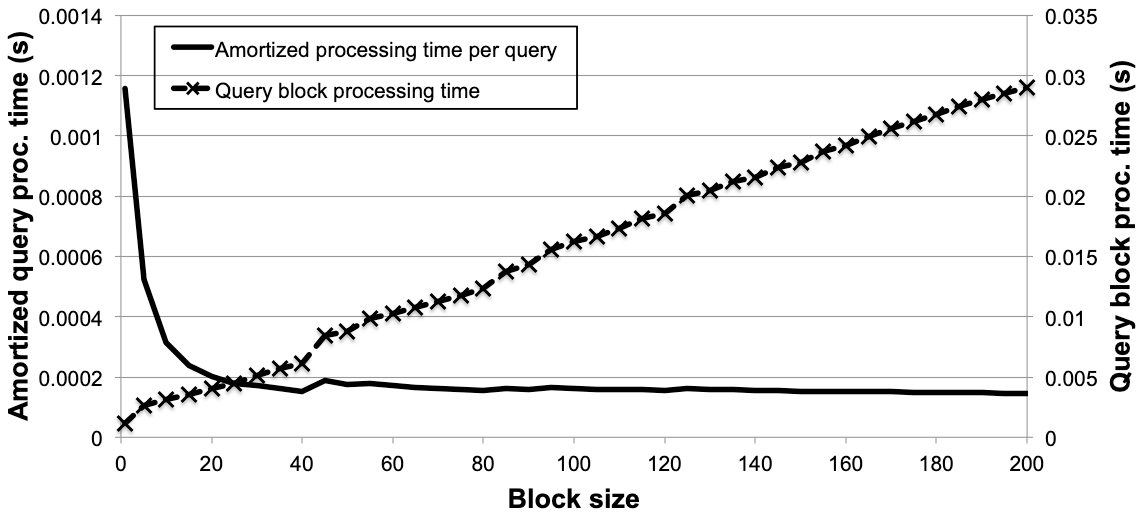
\includegraphics[width=\columnwidth]{figs/time-per-query-george.png}}
%\caption{Query block and amortized query processing times.}
%\label{fig:time_per_query}
%\end{figure}

In essence, we want to minimize the query response time given 
by: $query\ response\ time = queue\ waiting\ time + processing\ time$ by choosing the 
appropriate block size. The block size that minimizes response time will 
vary according to the system load that fluctuates during the execution. For instance,
when the load is low, the queue waiting time tends to be negligible and a small block 
size would minimize the processing time and, consequently, the response time. 
As the load increases, the queue waiting time will grow, and the block size 
should increase accordingly to improve the throughput and minimize the waiting 
time or penalty due to congestion in the input query queue~\cite{Menasce:2001:CPW:560806}. 
%In this case, the processing time will increase due to the larger block size
%grouped for execution in a single GPU call, but the better throughput will avoid
%a higher penalty due to a congestion in the input query queue~\cite{Menasce:2001:CPW:560806}.



%When queries arrive at the search node, we could just search for them, one by one, as they arrive. However, 
%this is very inefficient, since transferring data to the GPU has high latency. If we process more than one 
%query at a time, we can amortize that latency. However, we are faced with the following question: how many 
%queries to search for at the same time? From now on, we will refer to the number of queries that we process 
%at the same time as the block size. 

%If the block size is too big, we might end up waiting too much time to gather the required number of queries, and, 
%as a consequence, the response time would suffer. On the other hand, if the block size is too small, then the high 
%latency of transferring data to the GPU becomes a problem. It’s also important to notice that the optimal block size 
%may vary with the query rate. If the query rate is high, we want bigger block sizes. If the query rate is low, we 
%want smaller block sizes. Since the query rate may vary along the time, it’s fundamental that any effective block 
%size control policy be dynamic.

%One simple block size control policy is: in a loop, execute all queries that are waiting in the input buffer together. Since when the query rate is small, the average block size is small, and when the query rate is big, the average block size is big, it might look like a good policy. However, it isn’t. 

%\begin{figure}[htbp]
%\centerline{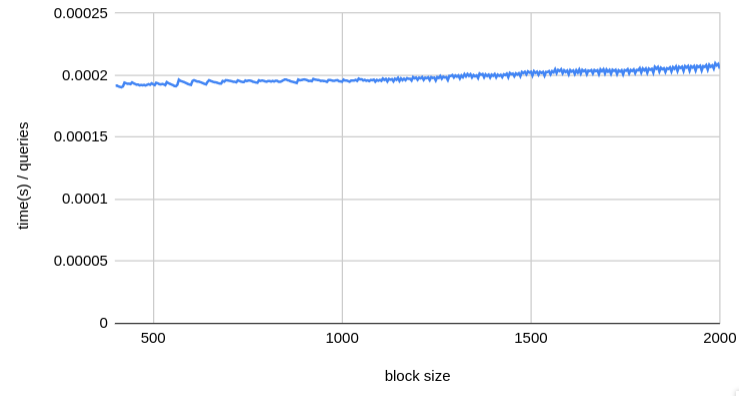
\includegraphics[scale=0.33]{figs/time_per_queries20k.png}}
%\caption{time / query vs block size}
%\label{fig:time_per_query20k}
%\end{figure}

% bad logic
%Figure~\ref{fig:time_per_query20k} helps explain why. As can be seen in the figure, while ever so slight, the time / query increases as the block size increases. While this increase may look insignificant, it actually isn't. Let's say that we are processing a block of 400 queries. However, for some reason, this block of queries took significantly more time than expected to execute. Therefore, we expect to have more than 400 queries in the input buffer after processing those 400 queries. However, since we have more queries, the time / query is increased as well, as can be seen in figure~\ref{fig:time_per_query20k}. Since the time / query has increased, it follows that it will take more time to process the queries, and, therefore, the number of queries waiting in the input buffer after processing this block will increase, which will increase the time / query, which will increase the number of queries waiting etc ad infinitum. Therefore, the system will run out of memory eventually and crash. This isn't just a theoretical analysis, we've implemented this policy, and we observed this behavior in practice. To avoid this problem, it is necessary to bound the block size by some threshold.



%If you look at the time / query chart (figure~\ref{fig:time_per_query}), you can notice roughly two regions:
% Maybe include a chart of the transfer time, though I feel that obtaining one that I feel 100% confident that is correct might be hard
%\begin{itemize}
%  \item \textbf{Bad region:} in this region, to the left of the vertical bar, the latency of the transfer to the GPU is huge when compared to the execution time. As we increase the number of queries, the time / query decreases, since the transfer cost is amortized.
%  \item \textbf{Stable region:} in this region, to the right of the vertical bar, the time / query is small and somewhat stable. The fixed cost of transfer to the GPU is insignificant next to the execution time.
%\end{itemize}
%
%Let’s say that the stable region begins at block size min$_$bs. Then, one way to deal with the problem described above would be to process all queries in the input buffer, up to min$_$bs queries. While this policy works, we found out experimentally that more sophisticated policies produce better results.

In order to adapt the GPU processing block size at runtime we proposed a strategy called Dynamic 
Query Processing Policy (DQPP). It decides that block size to use based on the 
size of the input query queue (IQQ), the observed query arrival rate (QAR), and expected GPU processing time for a given block size. The QAR is computed dividing the number of 
queries arriving in the system by the time interval between subsequent calls to 
the GPU. The GPU processing times for different block sizes are obtained in an 
offline benchmark run and are stored in the table of processing times (TPT) with an 
entry per size. We also use the block size with maximum throughput (BSMT), which
is computed from TPT.


%In order to address these challenges,
%%%discussed before, in this paper we propose a policy that modifies the block size at runtime. The decision about the block size to use is based on
%size of the input query queue (IQQ), the observed query arrival rate (QAR), and expected GPU processing time for a given block size. The
%first component is obtained by probing the queue. The QAR is computed by dividing the number of queries arriving in the system
%from subsequent calls to the GPU. The GPU processing time is obtained in an offline benchmark run in which the block size
%is varied and the associated execution time is recorded. The size is increased until the GPU has no more  memory available
%to process the input queries. This results in a table of processing times (TPT) with an entry per size. The profiling is 
%performed only once per GPU and is important to make the solution portable to GPUs with different performance/architectures. We 
%also compute the block size with maximum throughput (BSMT) to use in our algorithm.

\begin{algorithm}[H]
\caption{Dynamic Query Processing Policy (DQPP)}
\begin{algorithmic}[1]
\While{$True$} 
    \State $IQQ.waitNotEmpty()$
    \State $L \gets IQQ.length$
    \If{$L \ge BSMT$} 
        \State $process(IQQ, BSMT)$
    \Else
        %\State $qae \gets TPT[ibuf.length]~/~eqi$
        \State $TTB \gets (BSMT - L) / QAR$
        
        \State $TFL \gets TPT[L] - TTB$
        
        \If{$TTB \times L < (BSMT - L) \times TFL$}
    	    \State $process(IQQ, L)$
    	\Else 
    	    \State $IQQ.WAIT(TTB, BSMT)$
    	    \State $process(IQQ, min(IQQ.length, BSMT))$
    	\EndIf
    \EndIf
\EndWhile
\end{algorithmic}
\label{alg:dynamic}
\end{algorithm}

Algorithm~\ref{alg:dynamic} presents the DQPP strategy. The main loop of the algorithm 
is executed by the GPU manager 
thread until there is work to do. It will block if IQQ is empty, as shown in line~2. If
there are queries to be processed, it may process a block of queries already received or wait for 
more to arrive. If the number of queries ready are sufficient to execute with the block 
size configuration that leads to the best throughput (BSMT), the algorithm dispatches BSMT queries 
for the GPU execution. Please note that making a call with a larger number of queries is
suboptimal as it would increase query processing of the queries in the block without
improving the throughput.

When the number of queries L in IQQ is smaller than BSMT, it 
decides whether waiting for more queries to
arrive to process a larger number of queries in a GPU call is more efficient than dispatching
the currently available queries for execution now. 
%This may happen
%when a substantial amount of queries is expected to arrive soon. In this case, executing the
%queries currently in the queue may lead to a waiting time of those queries that will arrive soon
%after the GPU is called. 
To decide whether it is worthwhile waiting, DQPP estimates the
weighted query waiting time increase in each case (wait or execute now), and selects
the smallest one. Line~7 of Algorithm~\ref{alg:dynamic} computes the time estimate to have
BSMT queries ready for execution that is the configuration with best efficiency. This is done
by dividing the number of queries that should be received in this case (BSMT-L) by the query 
arrival rate (QAR). This is the additional waiting time that the L queries ready to execute would 
pay to wait.

On the other hand, if the GPU executes now with the L queries available, the ones arriving in the interval
between the GPU call and its return will sit waiting in the queue. Then DQPP has to decide which waiting time
weighted by the number of queries in each case is smaller. It then compute TFL that is the time interval
between the BSMT-L are queries received and the GPU finishes the execution of the L queries. Please
notice that if TFL is smaller than zero, it means that the execution of the L queries will end before BSMT-L are received. Thus, it is obvious that the L queries should be dispatched for execution
now. Further, having computed the waiting time of the L queries (TTB) and the one of the BSMT-L queries (TFL), they
are multiplied by the number of queries to select the smallest weighted waiting time (line~9). If processing the currently queued queries is the best option line~10 is executed. Otherwise, the system will
wait for TBB units of time or until IQQ.length (L) $<$ BSMT, whatever occurs first, and 
process the queries queued, even if its is smaller than BSMT.

